% !Rnw weave = knitr
% The Data
\section{The Data}
\label{sec:thedata}


The data was collected following the floods in Pakistan in 2010. Small Changes.

It surveyed affected villages in GB, KPK, Punjab and Sindh.

% make code to plot Vill distribution but don't run or show it.



The distribution of villages within Tehsils within Provinces is seen in Figure~\ref{fig:VillageDist}.

\begin{figure}[!hbtp]
\begin{knitrout}
\definecolor{shadecolor}{rgb}{1, 1, 1}\color{fgcolor}\begin{kframe}


{\ttfamily\noindent\textcolor{warningcolor}{\#\# Warning: 'opts' is deprecated.\\\#\# Use 'theme' instead.\\\#\# See help("Deprecated")}}

{\ttfamily\noindent\textcolor{warningcolor}{\#\# Warning: 'theme\_text' is deprecated.\\\#\# Use 'element\_text' instead.\\\#\# See help("Deprecated")}}\end{kframe}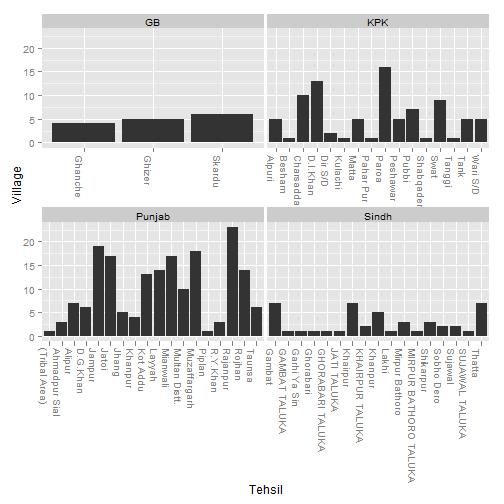
\includegraphics[width=.9\linewidth]{thedata/figures/VillDistPlot} 
\end{knitrout}

\caption{Distribution of villages within Tehsils within the four Provinces.\label{fig:VillageDist}}
\end{figure}

Here is the code to run it.

\begin{knitrout}
\definecolor{shadecolor}{rgb}{1, 1, 1}\color{fgcolor}\begin{kframe}
\begin{alltt}
\hlfunctioncall{ggplot}(vills, \hlfunctioncall{aes}(x = Tehsil)) + \hlfunctioncall{geom_bar}(\hlfunctioncall{aes}(y = Village), stat = \hlstring{"identity"}) + 
    \hlfunctioncall{opts}(axis.text.x = \hlfunctioncall{theme_text}(angle = 270, hjust = 0)) + \hlfunctioncall{facet_wrap}(~Province, 
    scales = \hlstring{"free_x"})
\end{alltt}
\end{kframe}
\end{knitrout}


The analysis begins in Section~\ref{sec:overall}.
